\section{Nice Graphs}
We call a graph $G:=(V, E)$ \emph{nice} if and only if it has the following properties

\begin{enumerate}
    \item \emph{reflexive} there is an self-edge for each vertex of $G$
    \item \emph{symmetric} if $(u,v)\in E$ then also $(v,u)\in E$
    \item \emph{equal weight} Each edge has the same weight.
\end{enumerate}

Without the loss of generality, for nice graphs we can set the weights to 1.

\begin{proof}[TODO talk about equivalent problems]
    There is an \emph{equivalent} problem with weights 1 for each nice graph.
\end{proof}

\begin{lemma}\label{close-press-button}
    Given a nice graph $G$, and an instance $L$ to the standard problem on $G$ with a solution $S$.

    For every lit button $b\in L$ there is a button $s\in S$ within $d(b,s) \leq 1$. 
\end{lemma}

\begin{proof}
    Assume the contrary. I.e. All buttons in the solution have a distance greater then 1 to all lit buttons of $L$. Since the effect of pressing a button has reach 1, no lit button in $L$ will change when pressing any $s\in S$.
    Contrary to $S$ being a solution.
\end{proof}

\begin{remark}
    Something more general is true. $G$ does not have to be a nice graph.
\end{remark}

\begin{lemma}\label{restricted-solution}
    Given a nice graph $G$

    A solution to the restricted problem on G exists if and only if a solution to the standard problem exists.
\end{lemma}

\begin{proof}
    $\Longleftarrow$ A solution to the restricted problem is also a solution to the standard problem.

    $\Longrightarrow$ We will use induction on the length of a solution to show that a solution $S$ to the standard problem on $G$ can be transformed to a solution $S'$ to the restricted problem on $G$.

    Assume all solution $S$ to the standard problem on $G$ with $|S| < k$ can be transformed to solution to the restricted problem. We will show that a solution $S$ with $|S| = k$ can also be transformed.
    Let $S$ with $|S| = k$ be given. There are two situations to consider.

    \begin{enumerate}
        \item\label{lit-button} $S$ contains a lit button.
        \item\label{no-lit-button} $S$ does not contain a lit button.
    \end{enumerate}

    Without loss of generality, if we are in situation \ref{lit-button}, we assume that the first button in $S$ we press is lit, since we can freely reorder the sequence of button presses in a solution for the standard problem.
    Since this button is lit we can press it. The remaining solution for the standard problem can be transformed to a solution to the restricted problem by the induction hypotheses.

    In situation \ref{no-lit-button} we can apply lemma \ref{close-press-button}. Pick a lit button $b$ and choose button $s\in S$ with $d(b, s) = 1$. Without loss of generality we can assume that $s$ is the first button in $S$.
    The following alternate press sequence allows us to press $s$ without altering the resulting light pattern. Assume $\state(b) = k$.

    \begin{enumerate}
        \item press button $b$ exactly $q-k$ times. Since $G$ is reflexive $b$ is now unlit. Since $d(b,s) = 1$ we find $s$ in state $\state(s) = q-k$ and therefor lit.
        \item press button $s$ which is possible because $s$ is lit. Since $G$ is symmetric $s$ effects $b$, so $b$ becomes lit.
        \item press button $b$ exactly $k$ times.
    \end{enumerate}

    Notice that this is a valid press sequence in the restricted problem. Furthermore button $b$ is pressed $q$ times, so it has not effected the resulting light pattern.
    More importantly the above sequence presses $s$.

    The remaining solution for the standard problem can again be transformed to a solution to the restricted problem by the induction hypotheses.

    So by induction we have shown that any solution to the standard problem on $G$ can be transformed to a solution to the restricted probem on $G$.
\end{proof}

\begin{corollary}\label{restricted-bound}
    Let $S$ be a solution to the standard problem and $S'$ the corresponding solution to the retricted problem.

    Then $|S'|\leq(q+1)|S|$.
\end{corollary}

\begin{proof}
    In the worst-case scenario we need to transform every $s\in S$ by our alternate press sequence. In each such transform we press $q+1$ buttons. 
\end{proof}

\begin{theorem}
    For a nice graph $G$ we have

    The existance and solution problems for the restricted Lights Out variant are in $P$.
\end{theorem}

\begin{proof}
    By lemma \ref{restricted-solution} there exist a solution to the restricted problem if and only if there exists a solution to the standard problem.
    By theorem \ref{standard-complexity} the existance of a solution for the standard problem is in $P$.

    The result for the restricted solution problem follows from theorem \ref{standard-complexity} a solutions to the standard problem can be found in polynomial time.
    By lemma \ref{restricted-solution} and corollary \ref{restricted-bound} it can be transformed in polynomial time to a solution for the restricted problem.
\end{proof}

In general, when our graph is not nice we loose the property that the solutions to the lit problem are equivalent to the standard problem.

\begin{figure}\label{figure:not-nice-counter-examples}
  \mbox{
    \subfigure[Not reflexive]{\includegraphics[width=0.30\textwidth]{image/not-reflexive.dot.pdf}}\label{counter-example:not-reflexive}
    \subfigure[Not Symmetric]{\includegraphics[width=0.30\textwidth]{image/not-symmetric.dot.pdf}}\label{counter-example:not-symmetric}
    \subfigure[Not same Weight]{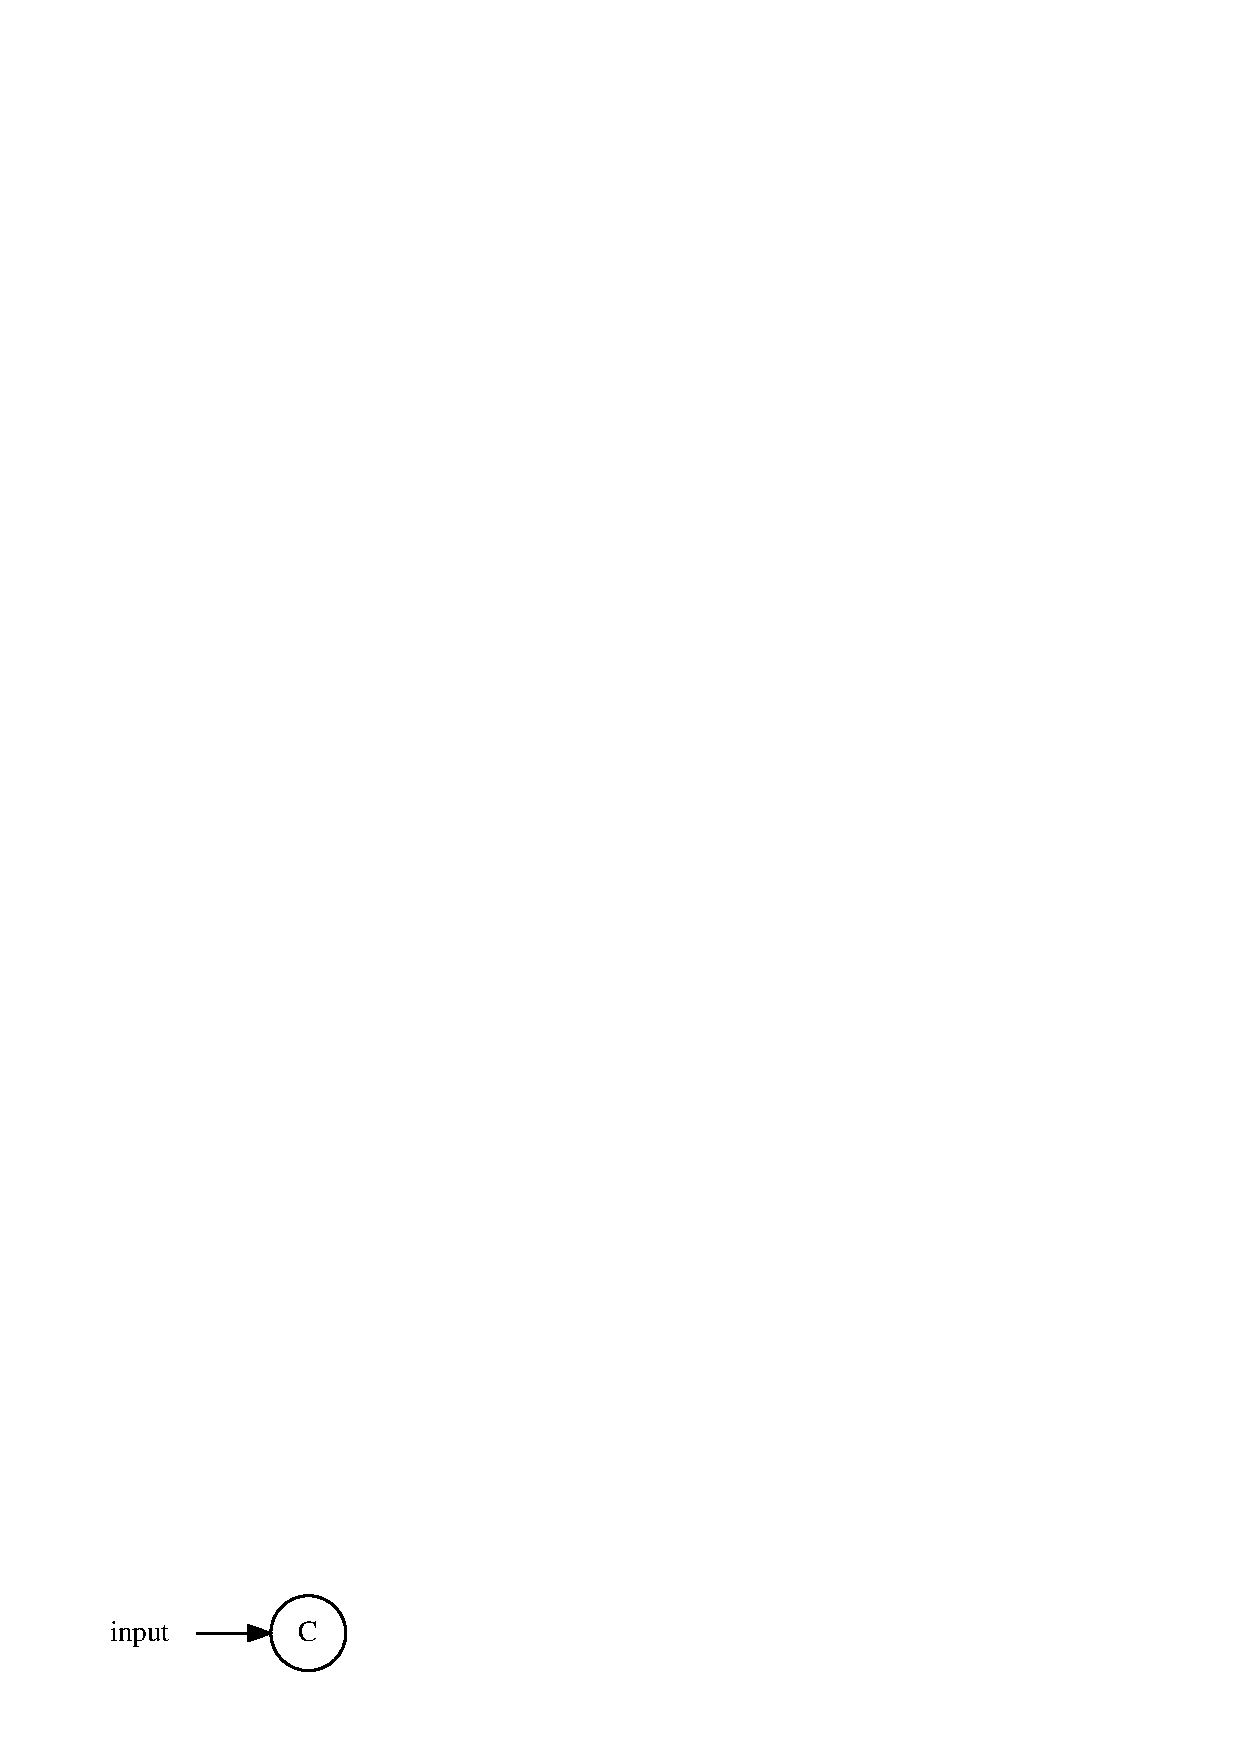
\includegraphics[width=0.30\textwidth]{image/c.dot.pdf}}\label{counter-example:not-same-weight}
   }
  \caption{Counter examples}
\end{figure}

\begin{remark}
    For the not reflexive counter example we have an $\state(a) = 0$ and $\state(b) = 1$. A standard solution is to press $a$, which can be achieved in lit problem.
    Pressing the only lit button results in $\state(a) = 1$, pressing any button in this state transforms back to the original or similar state.

    For the not symmetric case with only $\state(b) = 1$ and the rest is off, we have a solution by pressing $c, d, e, a$. Since neither of $c$, $d$, or $e$ is lit, and will never be lit this solution can not be transfered from the standard problem to the lit problem.
\end{remark}